\section{Développement firmware} \label{sec:Dev-firmware}

Lors de cette section, nous décrirons le processus de développement du firmware du PIC32. Les décisions prises seront expliquées et les différents algorithmes seront illustrés et décrits.


\subsection{Protocoles du GNSS} \label{ssec:ProtocolGNSS}
Il existe différents protocoles pour le format de données de localisation. Le \textbf{CAM-M8C-0} supporte plusieurs protocoles, visibles sur la figure \ref{fig:protocolsGNSS} :

\begin{figure}[h]
	\centering
	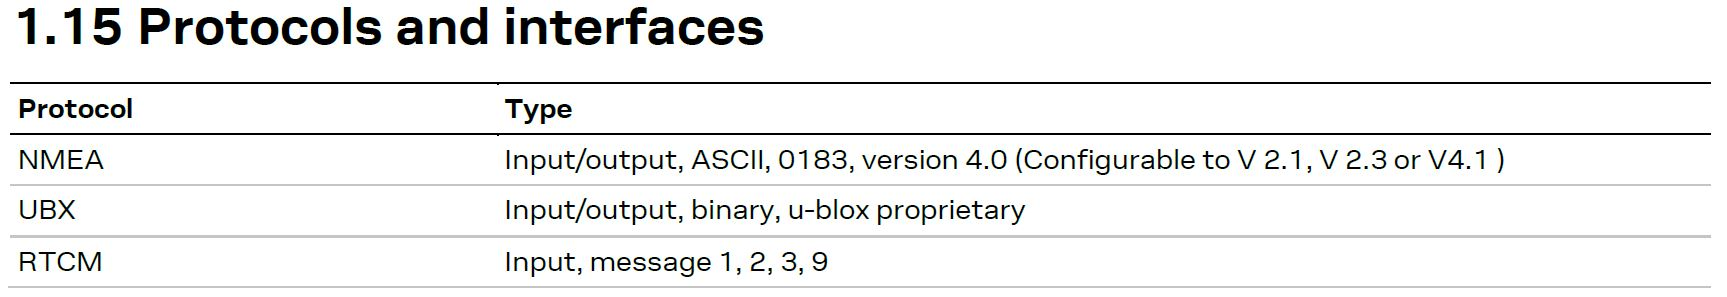
\includegraphics[width=.8\linewidth]{../figures/code/Protocols}
	\caption{Protocoles disponibles.}
	\source{\Gls{datasheet} du \href{https://content.u-blox.com/sites/default/files/CAM-M8-FW3\_DataSheet\_\%28UBX-15031574\%29.pdf}{CAM-M8C-0}}
	\label{fig:protocolsGNSS}
\end{figure}

\begin{tabularx}{\textwidth}{llX}
	\textbf{NMEA}& : & Norme établie par la \textit{National Marine Electronics Association}. Elle suit un format \fbox{\textbf{ASCII}}. \\
	\textbf{UBX} & : & Format propriétaire de u-blox avec des données \fbox{\textbf{binaires}}. Il permet d'envoyer des trames de configuration. \\
	\textbf{RTCM} & : & Protocole pour des données GPS différentielles. Établi par la \textit{Radio Technical Commission for Maritime Service}.
\end{tabularx} 


Le \textbf{CAM-M8C-0} est configuré, par défaut, pour envoyer des messages au format NMEA, comme illustré sur la figure \ref{fig:default-messages}.

\begin{figure}[!h]
	\centering
	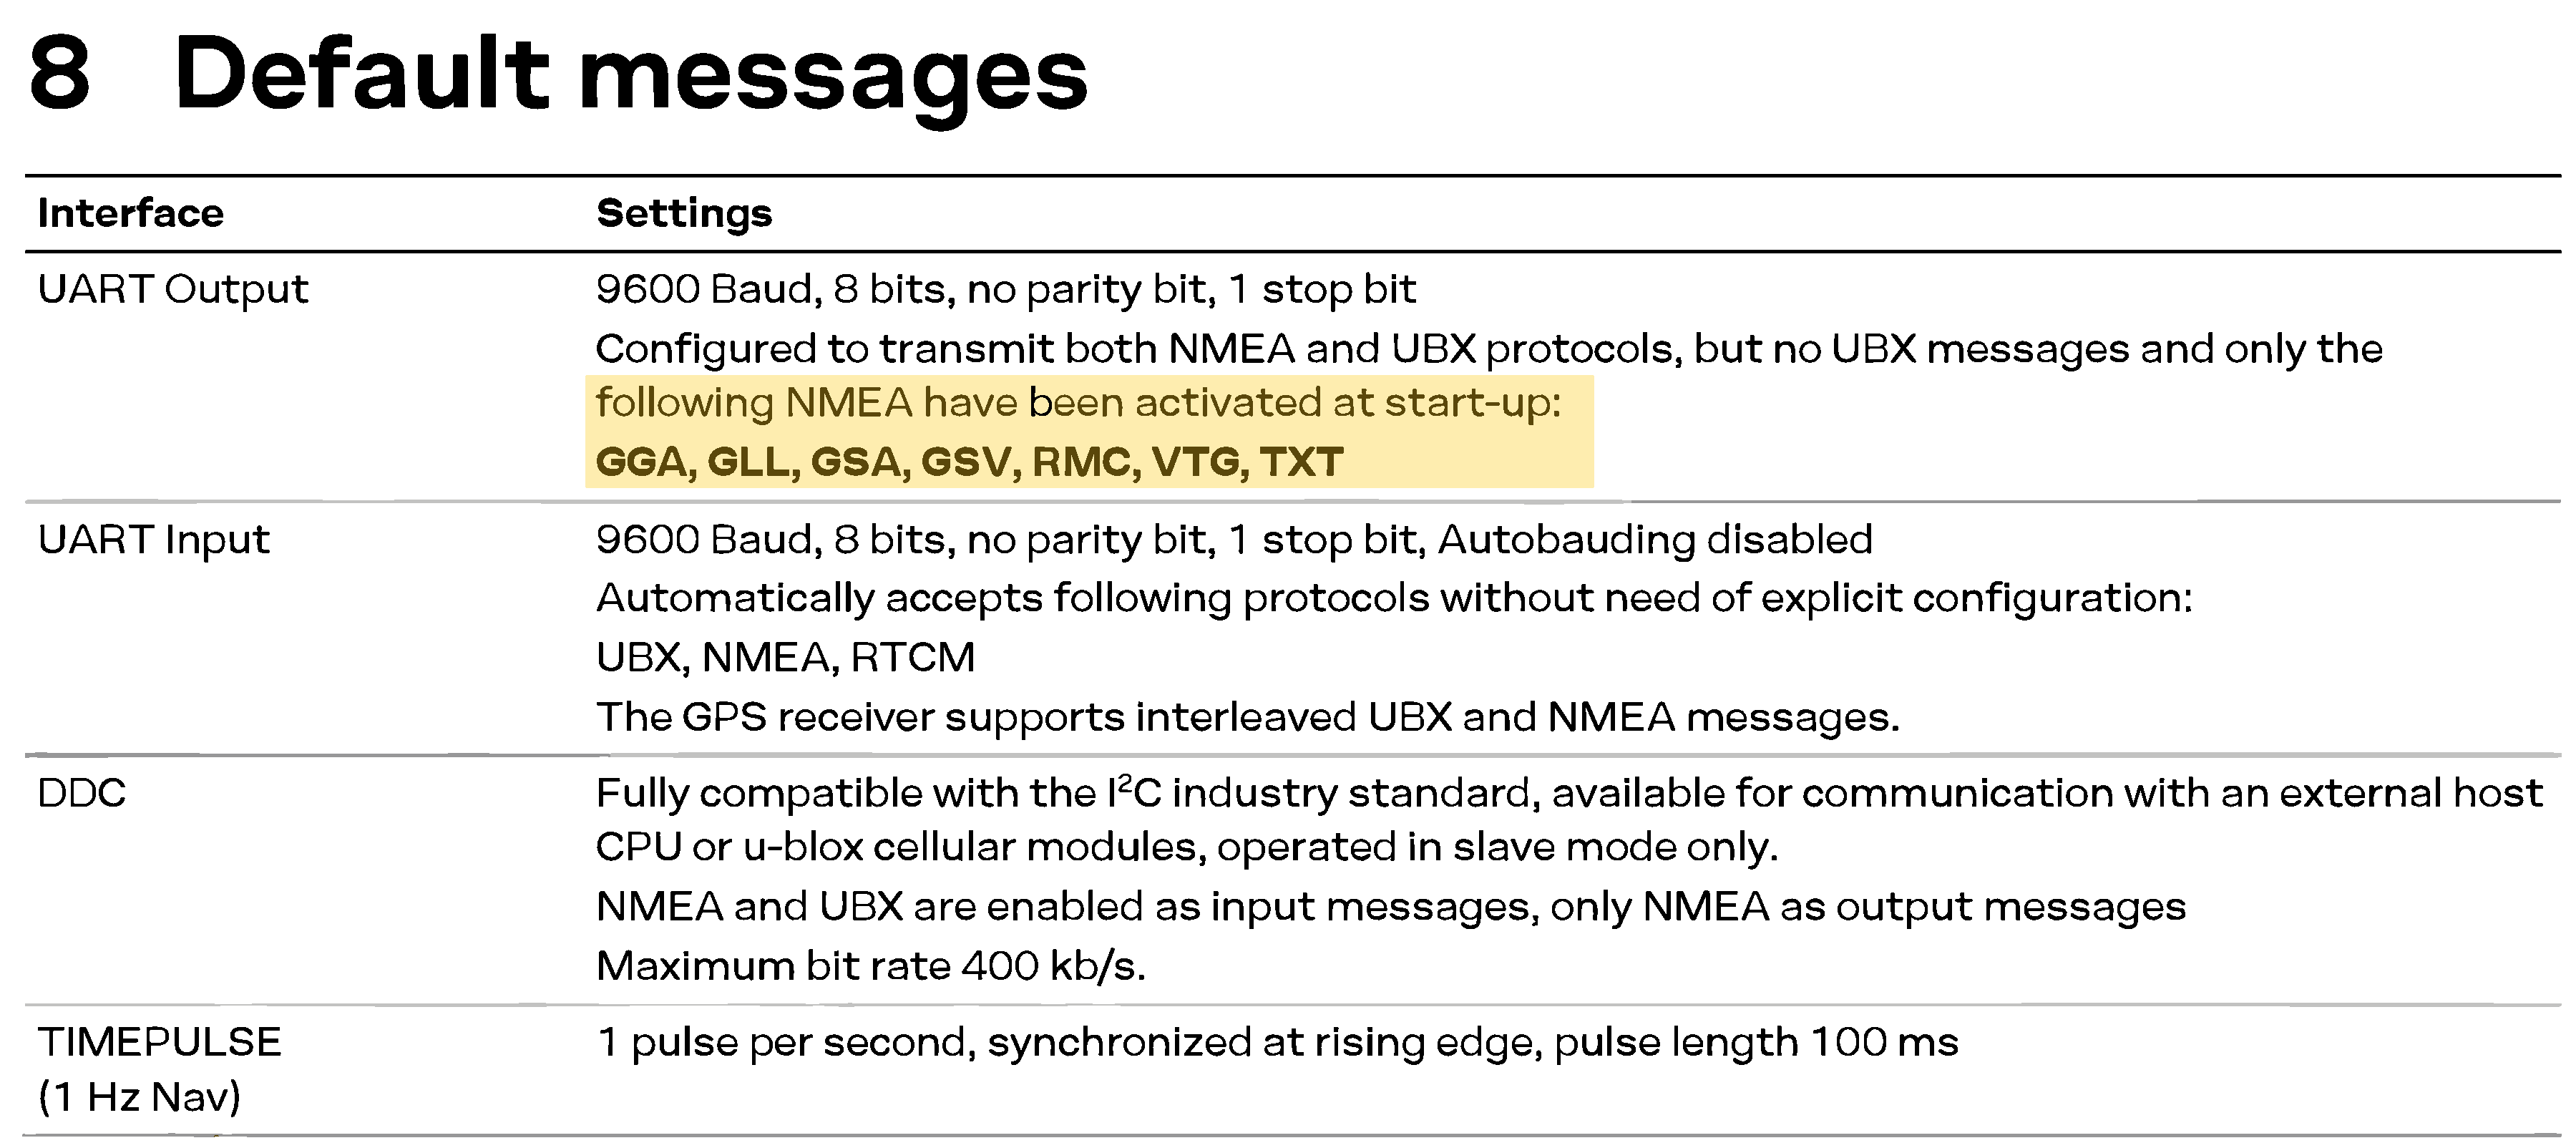
\includegraphics[width=0.8\linewidth]{../figures/code/Default-messages}
	\caption{Protocole par défaut.}
	\source{\Gls{datasheet} du \href{https://content.u-blox.com/sites/default/files/CAM-M8-FW3\_DataSheet\_\%28UBX-15031574\%29.pdf}{CAM-M8C-0}}
	\label{fig:default-messages}
\end{figure}

\clearpage

\subsubsection{Messages NMEA}
Comme nous avons pu constater sur la figure \ref{fig:default-messages}, il y a plusieurs messages \textbf{NMEA} : 

\textbf{GGA, GLL, GSA, GSV, RMC, VTG, TXT}

Celles-ci sont décrites dans le \href{https://www.ekf.de/c/cgps/cg2/inf/nmea_reference_manual.pdf}{manuel de référence du protocole NMEA} sur la figure \ref{fig:messages-nmea}

\begin{figure}[h]
	\centering
	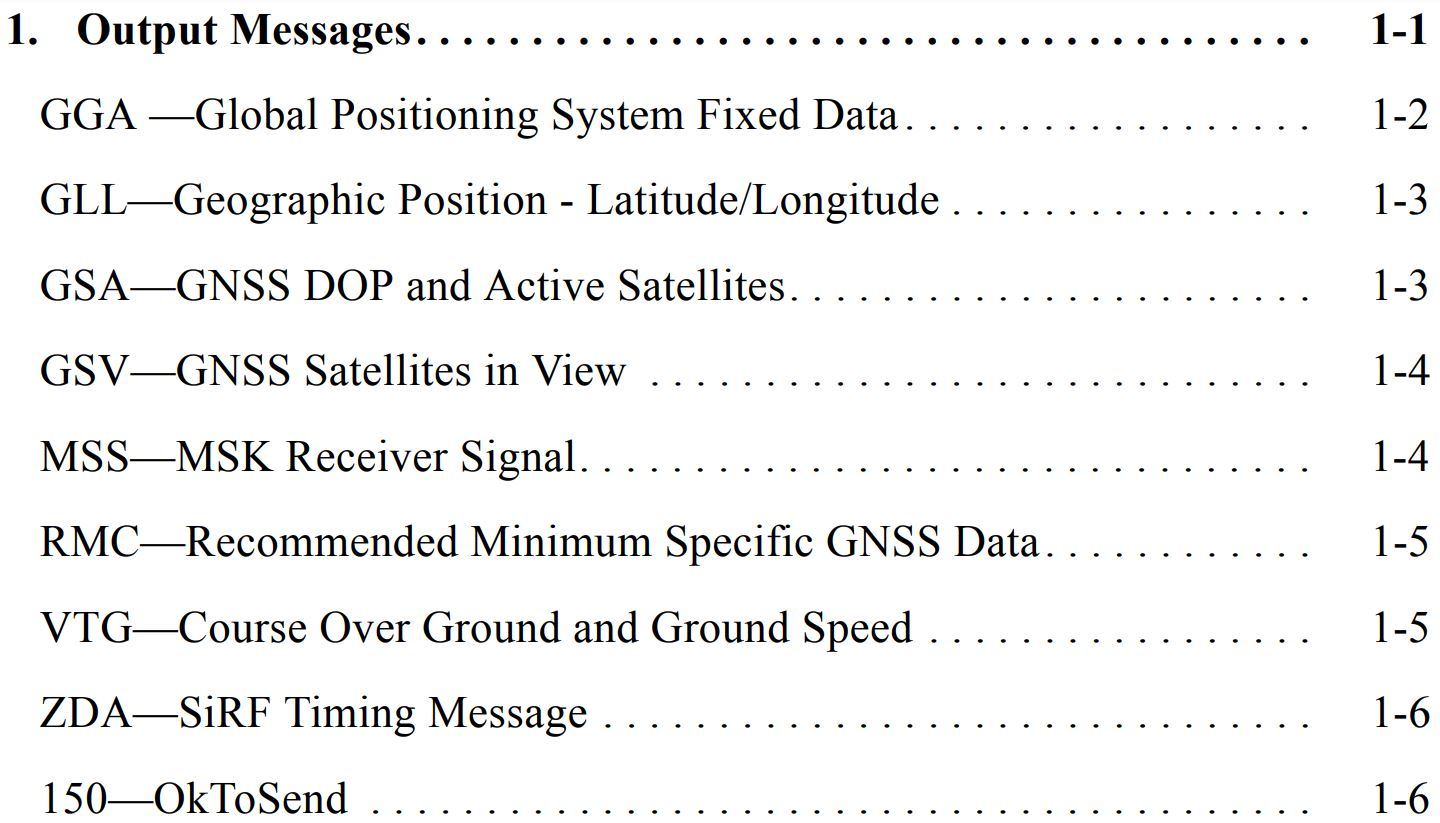
\includegraphics[width=0.55\linewidth]{../figures/code/Messages-NMEA}
	\caption{Messages NMEA.}
	\source{\href{https://www.ekf.de/c/cgps/cg2/inf/nmea_reference_manual.pdf}{Manuel du protocole NMEA}}
	\label{fig:messages-nmea}
\end{figure}

Les différents messages de la figure \ref{fig:messages-nmea} présentent des différentes données sous divers formats. Les messages peuvent être activés ou désactivés en configurant le module u-blox

\subsubsection{Interprétation des données NMEA}
Avant d'avoir le \gls{pcb} monté et exploitable, sachant que nous connaissons le protocole par défaut du module, nous pouvons analyser des données \textbf{NMEA} pour mieux les comprendre et les traiter par la suite. Pour se faire, le site \href{https://www.nmeagen.org/}{https://www.nmeagen.org/}, permet de générer des coordonnées GPS en format \textbf{NMEA}.

\begin{figure}[h]
	\centering
	\includegraphics[width=.75\textwidth]{../figures/code/map-localisation}
	\caption{Application d'une localisation NMEA.}
	\source{\href{https://www.nmeagen.org/}{nmeagen.org}, aéroport de La Blécherette, Lausanne}
	\label{fig:map-localisation}
\end{figure}

Sur la figure \ref{fig:parsed-nmea}, les messages de la figure \ref{fig:map-localisation} sont décodés.

\begin{figure}[h]
	\centering
	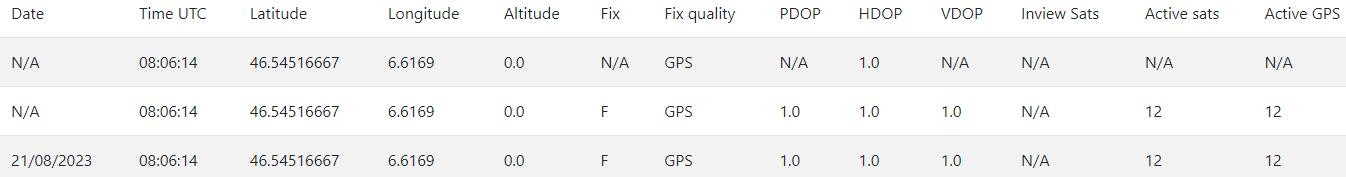
\includegraphics[width=0.8\linewidth]{../figures/code/parsed-nmea}
	\caption{Messages NMEA décodés.}
	\source{\href{https://swairlearn.bluecover.pt/nmea_analyser}{NMEA online analyser}}
	\label{fig:parsed-nmea}
\end{figure}

\clearpage

\subsubsection{Code décodeur de trame NMEA}

